% Options for packages loaded elsewhere
\PassOptionsToPackage{unicode}{hyperref}
\PassOptionsToPackage{hyphens}{url}
%
\documentclass[
]{book}
\usepackage{lmodern}
\usepackage{amssymb,amsmath}
\usepackage{ifxetex,ifluatex}
\ifnum 0\ifxetex 1\fi\ifluatex 1\fi=0 % if pdftex
  \usepackage[T1]{fontenc}
  \usepackage[utf8]{inputenc}
  \usepackage{textcomp} % provide euro and other symbols
\else % if luatex or xetex
  \usepackage{unicode-math}
  \defaultfontfeatures{Scale=MatchLowercase}
  \defaultfontfeatures[\rmfamily]{Ligatures=TeX,Scale=1}
\fi
% Use upquote if available, for straight quotes in verbatim environments
\IfFileExists{upquote.sty}{\usepackage{upquote}}{}
\IfFileExists{microtype.sty}{% use microtype if available
  \usepackage[]{microtype}
  \UseMicrotypeSet[protrusion]{basicmath} % disable protrusion for tt fonts
}{}
\makeatletter
\@ifundefined{KOMAClassName}{% if non-KOMA class
  \IfFileExists{parskip.sty}{%
    \usepackage{parskip}
  }{% else
    \setlength{\parindent}{0pt}
    \setlength{\parskip}{6pt plus 2pt minus 1pt}}
}{% if KOMA class
  \KOMAoptions{parskip=half}}
\makeatother
\usepackage{xcolor}
\IfFileExists{xurl.sty}{\usepackage{xurl}}{} % add URL line breaks if available
\IfFileExists{bookmark.sty}{\usepackage{bookmark}}{\usepackage{hyperref}}
\hypersetup{
  pdftitle={Biostatistics Portfolio II},
  pdfauthor={Dr.~F.J. Rodenburg   © 2021 Leiden University},
  hidelinks,
  pdfcreator={LaTeX via pandoc}}
\urlstyle{same} % disable monospaced font for URLs
\usepackage{color}
\usepackage{fancyvrb}
\newcommand{\VerbBar}{|}
\newcommand{\VERB}{\Verb[commandchars=\\\{\}]}
\DefineVerbatimEnvironment{Highlighting}{Verbatim}{commandchars=\\\{\}}
% Add ',fontsize=\small' for more characters per line
\usepackage{framed}
\definecolor{shadecolor}{RGB}{248,248,248}
\newenvironment{Shaded}{\begin{snugshade}}{\end{snugshade}}
\newcommand{\AlertTok}[1]{\textcolor[rgb]{0.94,0.16,0.16}{#1}}
\newcommand{\AnnotationTok}[1]{\textcolor[rgb]{0.56,0.35,0.01}{\textbf{\textit{#1}}}}
\newcommand{\AttributeTok}[1]{\textcolor[rgb]{0.77,0.63,0.00}{#1}}
\newcommand{\BaseNTok}[1]{\textcolor[rgb]{0.00,0.00,0.81}{#1}}
\newcommand{\BuiltInTok}[1]{#1}
\newcommand{\CharTok}[1]{\textcolor[rgb]{0.31,0.60,0.02}{#1}}
\newcommand{\CommentTok}[1]{\textcolor[rgb]{0.56,0.35,0.01}{\textit{#1}}}
\newcommand{\CommentVarTok}[1]{\textcolor[rgb]{0.56,0.35,0.01}{\textbf{\textit{#1}}}}
\newcommand{\ConstantTok}[1]{\textcolor[rgb]{0.00,0.00,0.00}{#1}}
\newcommand{\ControlFlowTok}[1]{\textcolor[rgb]{0.13,0.29,0.53}{\textbf{#1}}}
\newcommand{\DataTypeTok}[1]{\textcolor[rgb]{0.13,0.29,0.53}{#1}}
\newcommand{\DecValTok}[1]{\textcolor[rgb]{0.00,0.00,0.81}{#1}}
\newcommand{\DocumentationTok}[1]{\textcolor[rgb]{0.56,0.35,0.01}{\textbf{\textit{#1}}}}
\newcommand{\ErrorTok}[1]{\textcolor[rgb]{0.64,0.00,0.00}{\textbf{#1}}}
\newcommand{\ExtensionTok}[1]{#1}
\newcommand{\FloatTok}[1]{\textcolor[rgb]{0.00,0.00,0.81}{#1}}
\newcommand{\FunctionTok}[1]{\textcolor[rgb]{0.00,0.00,0.00}{#1}}
\newcommand{\ImportTok}[1]{#1}
\newcommand{\InformationTok}[1]{\textcolor[rgb]{0.56,0.35,0.01}{\textbf{\textit{#1}}}}
\newcommand{\KeywordTok}[1]{\textcolor[rgb]{0.13,0.29,0.53}{\textbf{#1}}}
\newcommand{\NormalTok}[1]{#1}
\newcommand{\OperatorTok}[1]{\textcolor[rgb]{0.81,0.36,0.00}{\textbf{#1}}}
\newcommand{\OtherTok}[1]{\textcolor[rgb]{0.56,0.35,0.01}{#1}}
\newcommand{\PreprocessorTok}[1]{\textcolor[rgb]{0.56,0.35,0.01}{\textit{#1}}}
\newcommand{\RegionMarkerTok}[1]{#1}
\newcommand{\SpecialCharTok}[1]{\textcolor[rgb]{0.00,0.00,0.00}{#1}}
\newcommand{\SpecialStringTok}[1]{\textcolor[rgb]{0.31,0.60,0.02}{#1}}
\newcommand{\StringTok}[1]{\textcolor[rgb]{0.31,0.60,0.02}{#1}}
\newcommand{\VariableTok}[1]{\textcolor[rgb]{0.00,0.00,0.00}{#1}}
\newcommand{\VerbatimStringTok}[1]{\textcolor[rgb]{0.31,0.60,0.02}{#1}}
\newcommand{\WarningTok}[1]{\textcolor[rgb]{0.56,0.35,0.01}{\textbf{\textit{#1}}}}
\usepackage{longtable,booktabs}
% Correct order of tables after \paragraph or \subparagraph
\usepackage{etoolbox}
\makeatletter
\patchcmd\longtable{\par}{\if@noskipsec\mbox{}\fi\par}{}{}
\makeatother
% Allow footnotes in longtable head/foot
\IfFileExists{footnotehyper.sty}{\usepackage{footnotehyper}}{\usepackage{footnote}}
\makesavenoteenv{longtable}
\usepackage{graphicx,grffile}
\makeatletter
\def\maxwidth{\ifdim\Gin@nat@width>\linewidth\linewidth\else\Gin@nat@width\fi}
\def\maxheight{\ifdim\Gin@nat@height>\textheight\textheight\else\Gin@nat@height\fi}
\makeatother
% Scale images if necessary, so that they will not overflow the page
% margins by default, and it is still possible to overwrite the defaults
% using explicit options in \includegraphics[width, height, ...]{}
\setkeys{Gin}{width=\maxwidth,height=\maxheight,keepaspectratio}
% Set default figure placement to htbp
\makeatletter
\def\fps@figure{htbp}
\makeatother
\setlength{\emergencystretch}{3em} % prevent overfull lines
\providecommand{\tightlist}{%
  \setlength{\itemsep}{0pt}\setlength{\parskip}{0pt}}
\setcounter{secnumdepth}{5}
\usepackage{booktabs}
\usepackage{amsthm}
\makeatletter
\def\thm@space@setup{%
  \thm@preskip=8pt plus 2pt minus 4pt
  \thm@postskip=\thm@preskip
}
\makeatother
\usepackage[]{natbib}
\bibliographystyle{plainnat}

\title{Biostatistics Portfolio II}
\author{Dr.~F.J. Rodenburg © 2021 Leiden University}
\date{}

\begin{document}
\maketitle

{
\setcounter{tocdepth}{1}
\tableofcontents
}
\hypertarget{preface}{%
\chapter*{Preface}\label{preface}}
\addcontentsline{toc}{chapter}{Preface}

This is the second part of the biostatistics portfolio. \href{https://fransrodenburg.github.io/Biostatistics-Portfolio-I/}{The first part} mainly served to ease you into the concepts and provide an introduction to programming in R. If you haven't followed the first part, at least make sure you \href{https://youtu.be/2Sovzf6lVRo}{install RStudio}.

This part aims to:

\begin{itemize}
\tightlist
\item
  Bridge the gap between year 1 and \href{https://fransrodenburg.github.io/General-Research-Skills/}{year 3};
\item
  Apply the methods that you have learned so far;
\item
  Show some actual analyses of real biological research.
\end{itemize}

You've now had one course in statistics, but probably little opportunity to ever put it to use. That is what this portfolio is hopefully going to address. Some chapters require you to use what you learned in year 1, others will show you some more advanced methods applied to data of courses you are currently following.

If you really want to understand every detail of analysis, consider pursuing a \href{https://www.universiteitleiden.nl/en/education/study-programmes/master/statistics--data-science}{degree in statistics}. For everyone else, just try and understand the gist of it, that is more than enough!

\begin{figure}
\includegraphics[width=1\linewidth]{figures/learninggoalstreeroots} \caption{In this part, some of the applications of statistics will be shown in the context of courses you are following at the IBL.}\label{fig:learninggoals}
\end{figure}

\begin{center}\rule{0.5\linewidth}{0.5pt}\end{center}

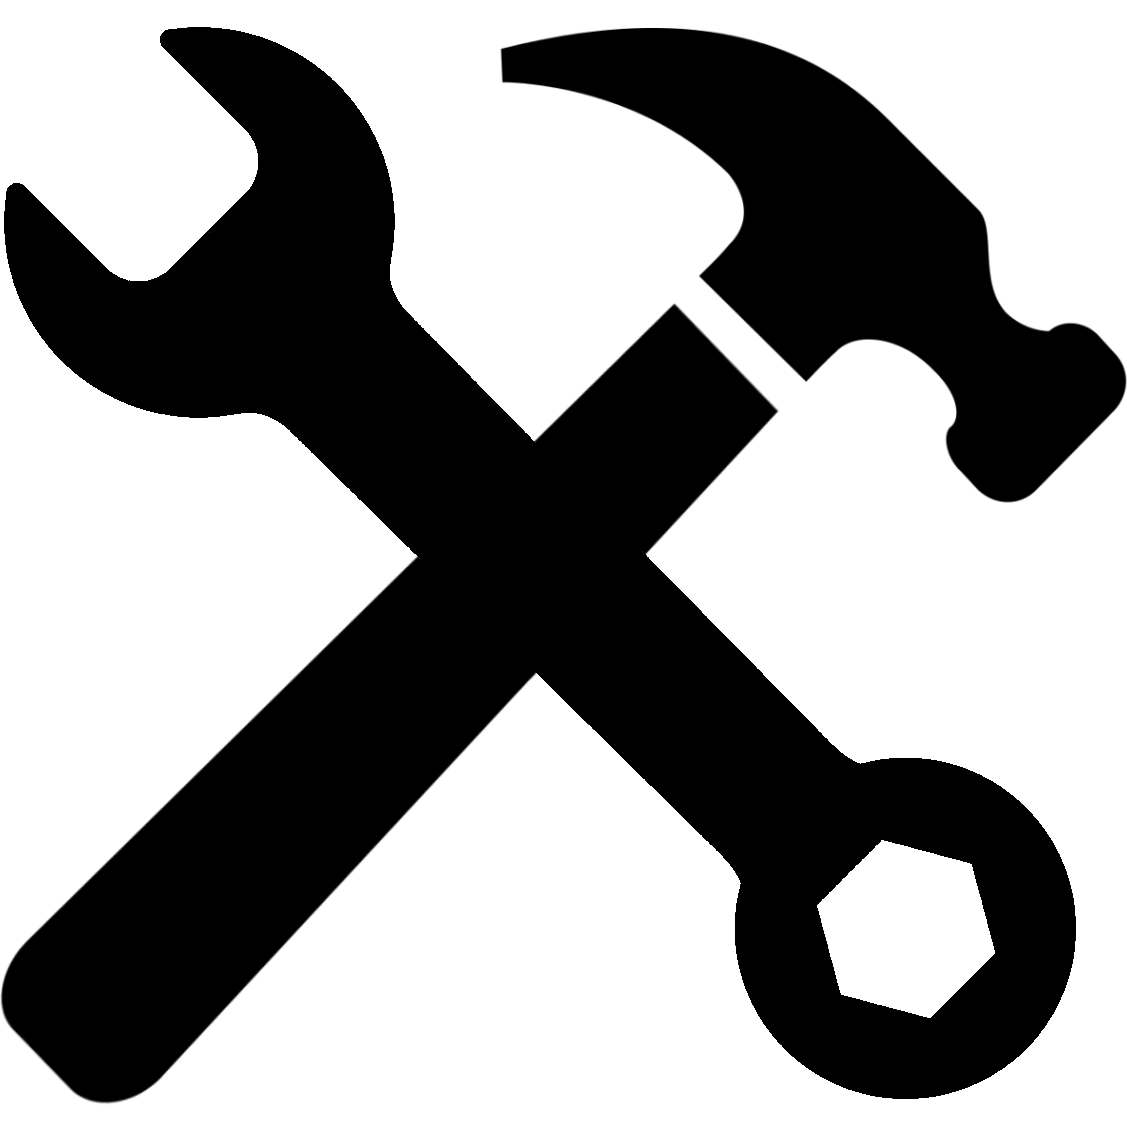
\includegraphics[width=0.20833in,height=0.20833in]{figures/underconstruction.png} The portfolio, as well as the online version of the course, are a work in progress. Please check back later for updates. Official information will always be communicated through Brightspace.

\hypertarget{bird-song}{%
\chapter{Bird Song}\label{bird-song}}

In this chapter, an advanced analysis is shown of the volume of different areas of the bird brain related to song. Your assignment is to read the explanation, have a look at the analysis used, and then perform \textbf{data cleaning} on your own data. Once your data is ready, copy the analysis and write a conclusion.

\begin{center}\rule{0.5\linewidth}{0.5pt}\end{center}

\hypertarget{introduction}{%
\section{Introduction}\label{introduction}}

Statistical analysis is about explaining the different sources of variance. A source of variance can be of interest, like the different areas of the brain, but it can also simply be a source of potential errors, like which student is performing the measurements, or which particular bird you are measuring. By correctly accounting for the different sources of variance, we end up with a powerful model that gives trustworthy standard errors and \(p\)-values.

In this analysis I want to demonstrate three things:

\begin{enumerate}
\def\labelenumi{\arabic{enumi}.}
\tightlist
\item
  \textbf{A complicated experimental design} like this one requires a complicated model called a mixed model;
\item
  \textbf{Comparing the groups with a mixed model} can fortunately still be fairly easy to do in R, and its results match up with the expectations.
\item
  \textbf{Data cleaning} is part of every analysis, and has a great impact on the results. This is the part you will be doing by yourself. The analysis you can then copy from my example.
\end{enumerate}

This chapter will demonstrate how (1) study design is a crucial part of scientific research, which dictates the type of model you should use; (2) even if you do not fully understand the (statistical) methods used in papers, you can still judge the validity of one's approach, and read the results; (3) even simple data cleaning can be a time-consuming task that requires careful consideration of how the data came to be.

Throughout this chapter I will use example data from a different year. You data should be (more or less) the same. Any differences you can iron out in the data cleaning assignment.

\hypertarget{a-complex-experimental-design}{%
\section{A Complex Experimental Design}\label{a-complex-experimental-design}}

The experiment consisted of measuring the total volume of different parts of the brain related to song. This experimental design has two difficulties that I want to address, before showing which model I used. Hopefully that will make it clear \emph{why} I used the model shown in the next paragraph, even if you are not familiar with it.

\hypertarget{braintransform}{%
\subsection{The Outcome Is Skewed}\label{braintransform}}

If a distribution has more deviations in one direction than the other, we call it \href{https://en.wikipedia.org/wiki/Skewness}{skewed}:

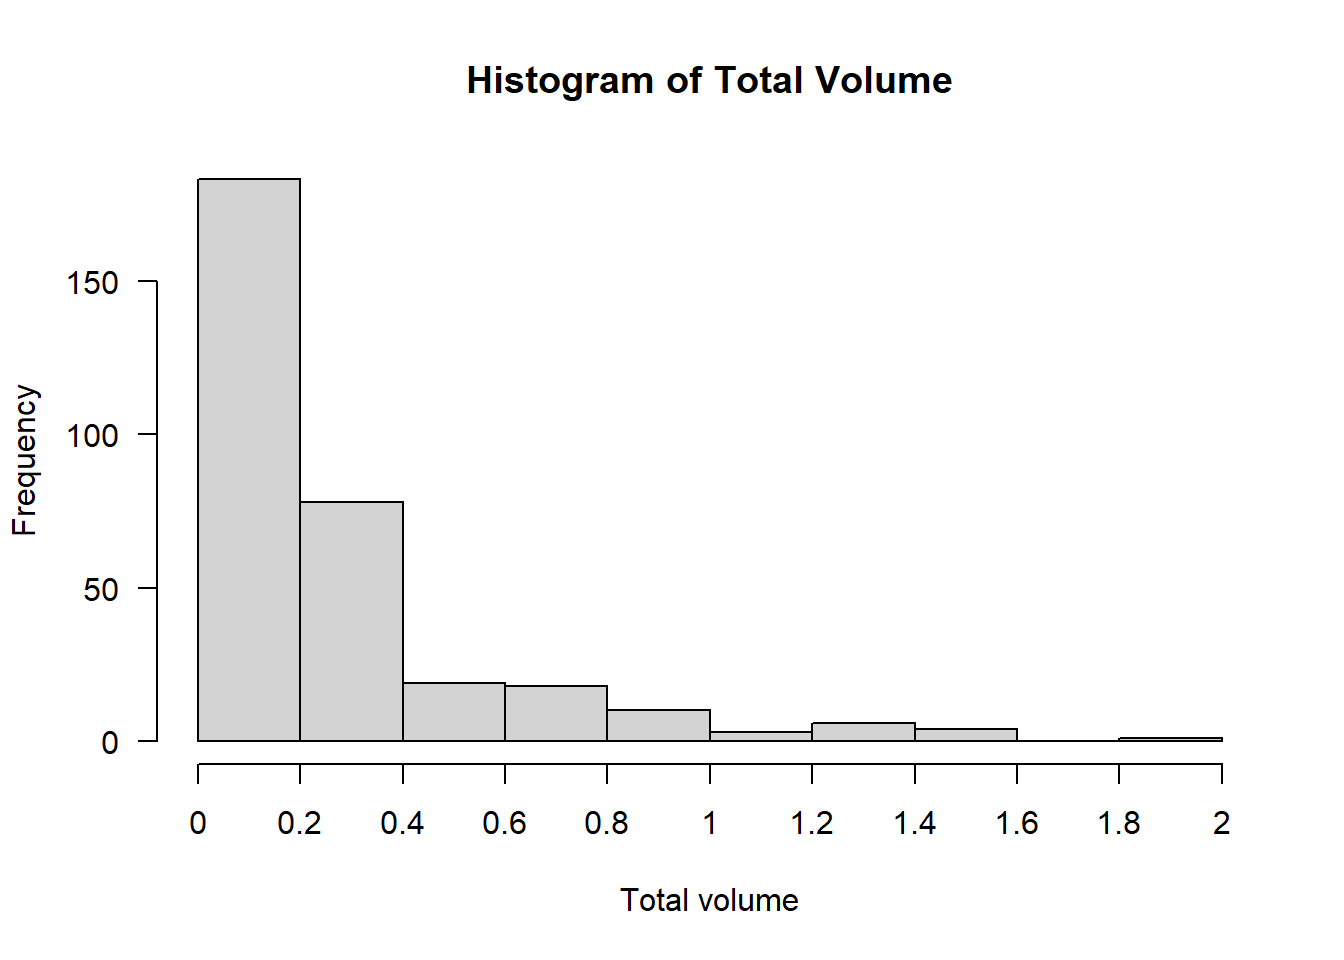
\includegraphics{Biostatistics_files/figure-latex/skewedbrain-1.pdf}

This histogram of the volume displays strong right-skew: Volumes of \(0\)--\(0.2\) are most common, \(0.2\)--\(0.4\) less common, and any larger volumes are exceedingly rare.

The model we're going to use in the next paragraph assumes (like many statistical tests and models) that if we account for the effects of the explanatory variables, what remains should be more or less \href{https://www.mathsisfun.com/data/standard-normal-distribution.html}{normally distributed} noise. With a response variable this strongly skewed, it is unlikely that assumption will hold. Even if we split by area of the brain, the distribution of volume is still right-skewed:

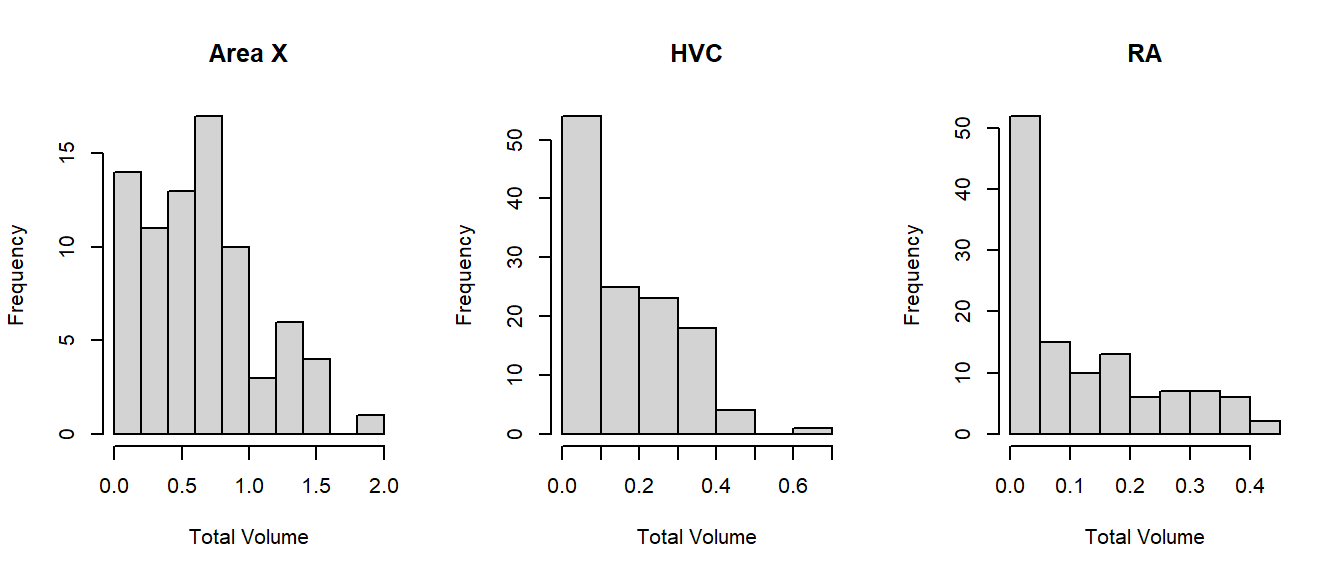
\includegraphics{Biostatistics_files/figure-latex/marginalbrain-1.pdf}

Why is volume so strongly right-skewed? Because the volume grows cubically (\(x^3\)): Volume is a three-dimensional measurement, determined by the length, width and depth. Therefore, we could consider \emph{transforming} the outcome as follows:

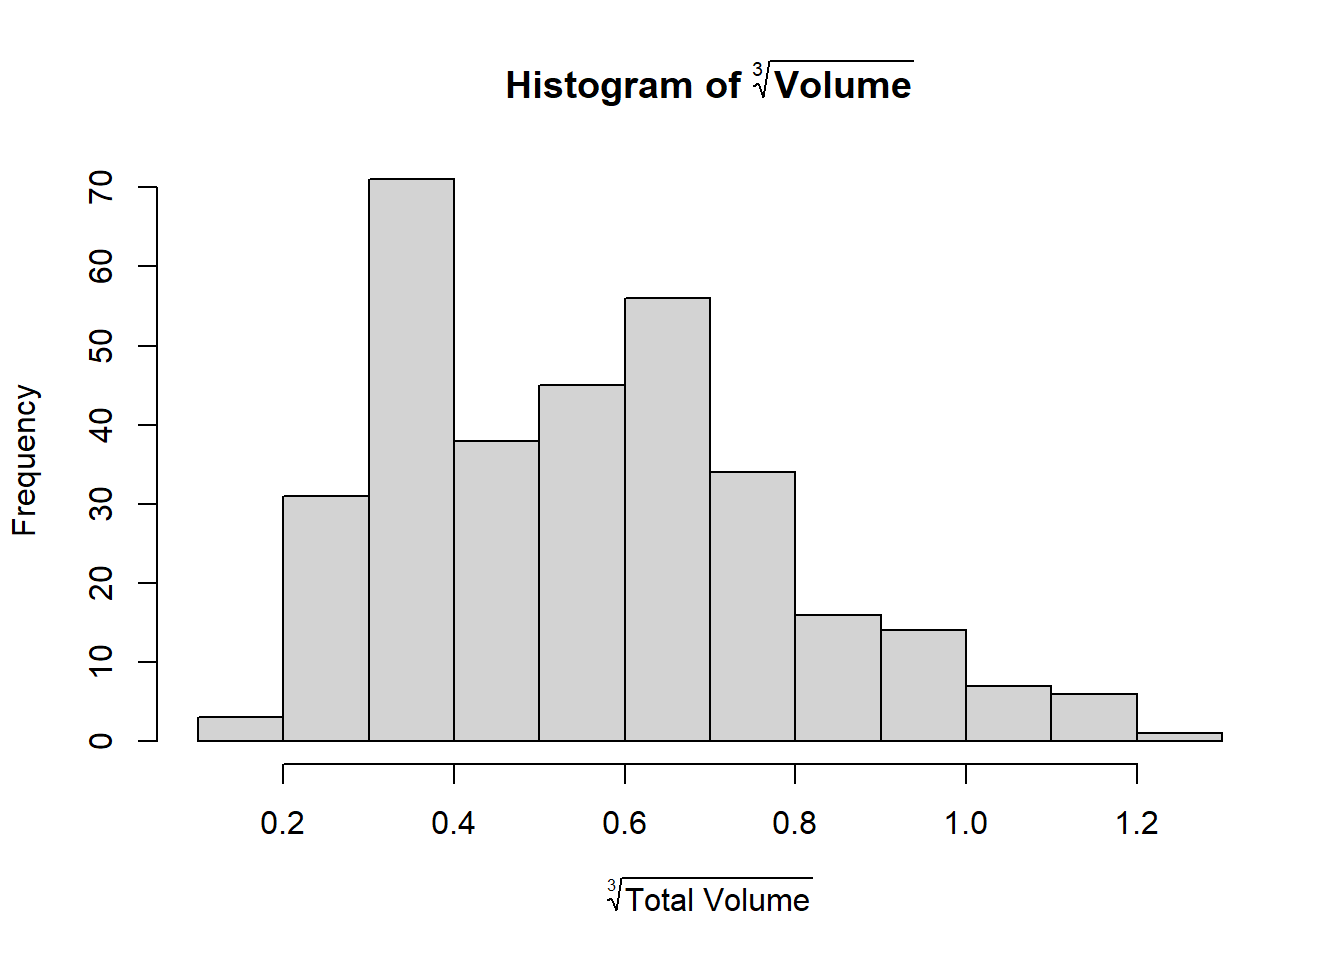
\includegraphics{Biostatistics_files/figure-latex/unskewedbrain-1.pdf}

We can also split by area again and see that there is indeed no more right-skew:

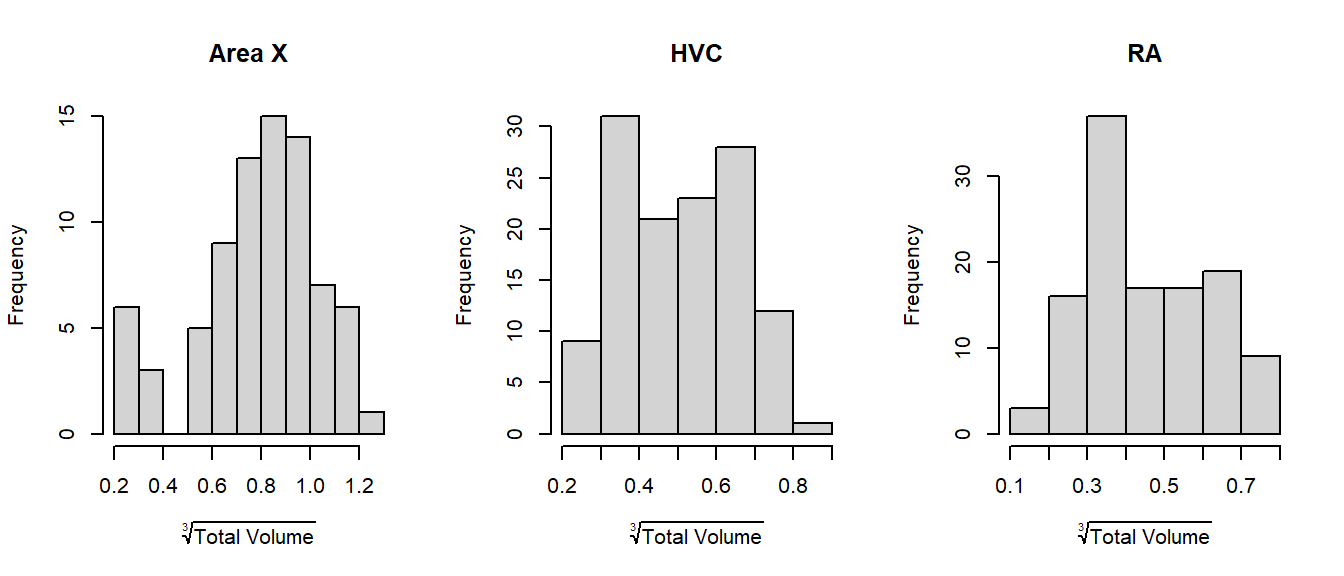
\includegraphics{Biostatistics_files/figure-latex/marginalunskewedbrain-1.pdf}

\hypertarget{braindependence}{%
\subsection{The Measurements are Dependent}\label{braindependence}}

\begin{figure}
\centering
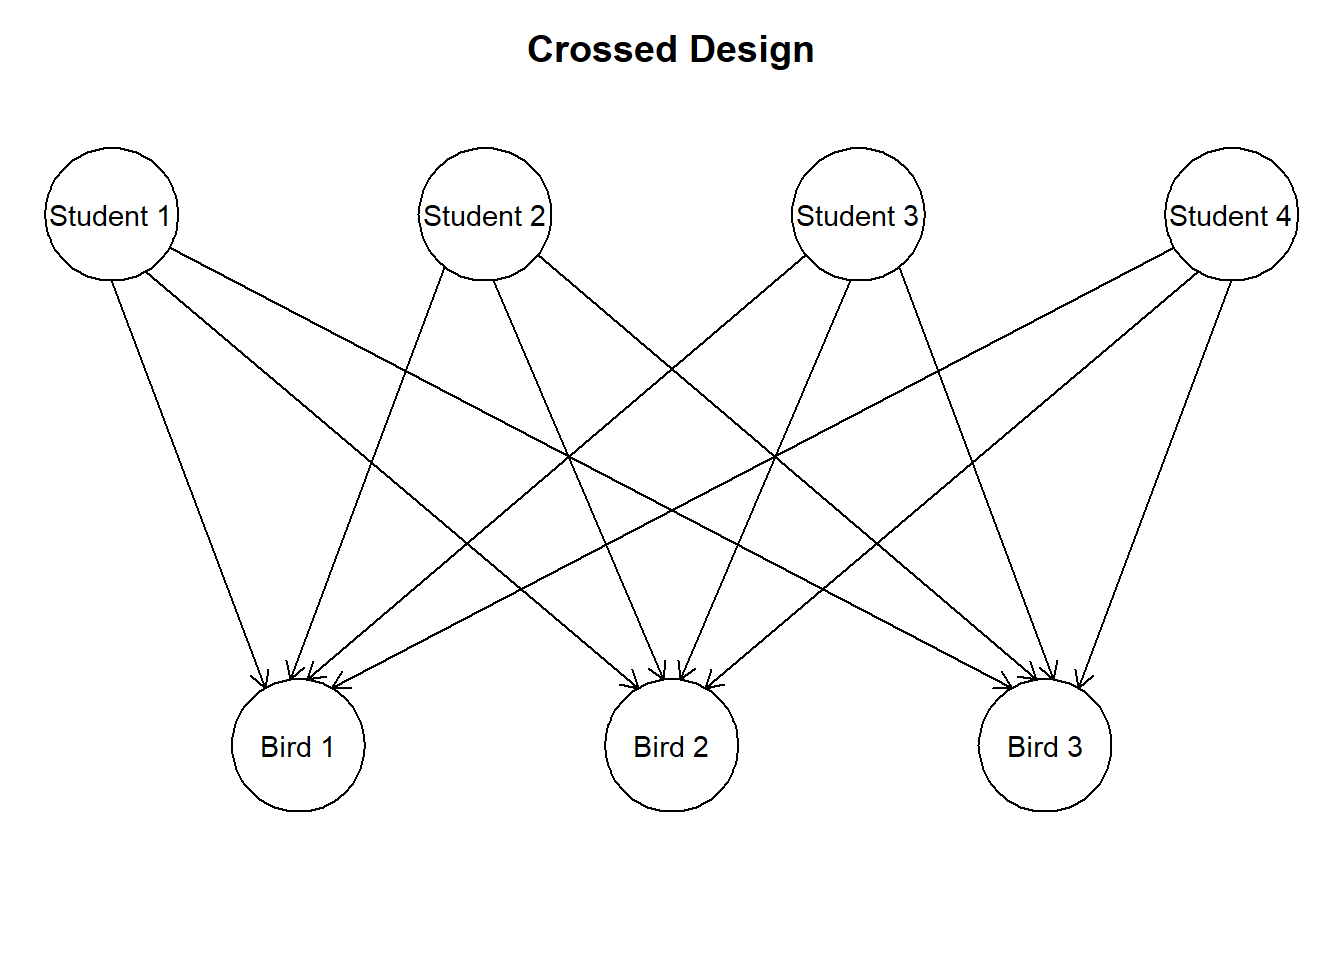
\includegraphics{Biostatistics_files/figure-latex/crossedrandomfig-1.pdf}
\caption{\label{fig:crossedrandomfig}\label{fig:crossedrandom}A simplified version of the experiment. Each bird has had different parts of its brain measured by different students.}
\end{figure}

Here is a very brief description of \textbf{the problem} and \textbf{the solution}:

\begin{itemize}
\tightlist
\item
  \textbf{Most tests and models assume independent measurements};
\item
  Each bird in the data set has been measured more than once (different brain areas). These measurements come from the same individual and are therefore, \textbf{measurements of the same bird are not independent};
\item
  In the first year's course about statistics you learned to \textbf{compare dependent data} through a paired \(t\)-test. A paired \(t\)-test can only compare two sets of paired measurements;
\item
  A more general way to deal with dependent data is \textbf{through a mixed model}.
\item
  This works \textbf{by estimating a random effect for birds}. This is like assuming that these birds come from some larger population of birds we could have used in the experiment. Instead of estimating a separate effect for each bird, we estimate the variance between birds and subtract the effect of the individual birds from the effects of interest.
\end{itemize}

Another potential source of dependence is\ldots{} you! No matter how hard we try to perform measurements according to protocol, there will always be minor, but systematic differences in the way each student performs the measurement. If each student performed one measurement, this would not pose any problem. However, as shown in figure \ref{fig:crossedrandom}, each student has performed several measurements. If the differences in measurement between students are sufficiently large, this poses a problem. Therefore, \textbf{measurements of the same student might be correlated}.

Fortunately, both problems can be tackled with the same solution: A \textbf{mixed model}.

\hypertarget{analysis-with-a-mixed-model}{%
\section{Analysis With a Mixed Model}\label{analysis-with-a-mixed-model}}

To fit a mixed model, we are going to use a package called \texttt{lmerTest}. The entire procedure then boils down to:

\begin{enumerate}
\def\labelenumi{\arabic{enumi}.}
\tightlist
\item
  Install package \texttt{lmerTest} if you don't have it;
\item
  Load package \texttt{lmerTest};
\item
  Fit a mixed model with \texttt{lmer()};

  \begin{itemize}
  \tightlist
  \item
    Use \protect\hyperlink{braintransform}{the transformation described above};
  \item
    Specify \protect\hyperlink{braindependence}{which variables cause the dependence}.
  \end{itemize}
\end{enumerate}

\hypertarget{install-package-lmertest}{%
\subsection{\texorpdfstring{Install Package \texttt{lmerTest}}{Install Package lmerTest}}\label{install-package-lmertest}}

\begin{Shaded}
\begin{Highlighting}[]
\KeywordTok{install.packages}\NormalTok{(}\StringTok{"lmerTest"}\NormalTok{)}
\end{Highlighting}
\end{Shaded}

\hypertarget{load-package-lmertest}{%
\subsection{\texorpdfstring{Load Package \texttt{lmerTest}}{Load Package lmerTest}}\label{load-package-lmertest}}

\begin{Shaded}
\begin{Highlighting}[]
\KeywordTok{library}\NormalTok{(}\StringTok{"lmerTest"}\NormalTok{)}
\end{Highlighting}
\end{Shaded}

\hypertarget{brainmodel}{%
\subsection{\texorpdfstring{Fit a Mixed Model With \texttt{lmer()}}{Fit a Mixed Model With lmer()}}\label{brainmodel}}

Let's call this model \texttt{model1}:

\begin{Shaded}
\begin{Highlighting}[]
\NormalTok{model1 <-}\StringTok{ }\KeywordTok{lmer}\NormalTok{(Volume}\OperatorTok{^}\NormalTok{(}\DecValTok{1}\OperatorTok{/}\DecValTok{3}\NormalTok{) }\OperatorTok{~}\StringTok{ }\NormalTok{Area }\OperatorTok{+}\StringTok{ }\NormalTok{Hemisphere }\OperatorTok{+}\StringTok{ }\NormalTok{(}\DecValTok{1} \OperatorTok{|}\StringTok{ }\NormalTok{BirdID) }\OperatorTok{+}\StringTok{ }\NormalTok{(}\DecValTok{1} \OperatorTok{|}\StringTok{ }\NormalTok{StudentID), }
               \DataTypeTok{data =}\NormalTok{ Birdsong)}
\end{Highlighting}
\end{Shaded}

\begin{itemize}
\tightlist
\item
  \texttt{lmer} is short for linear mixed effects regression---a mixed model;
\item
  \texttt{Volume} is transformed as \(\sqrt[3]{x} = x^{\frac{1}{3}}\) \protect\hyperlink{braintransform}{as explained earlier};
\item
  \texttt{Area} and \texttt{Hemisphere} are the effects of interest;
\item
  Using the \texttt{(1\ \textbar{}\ ...)} notation, I am telling the function I want to estimate the variance between birds and the variance between students;
\item
  Using the \texttt{data} argument, I am telling the function where to find all these variables.
\end{itemize}

That's the whole model! You might not have been able to think of that yourself, but if you understand why this particular model was used, that is more than enough.

\hypertarget{interpreting-the-output}{%
\subsection{Interpreting the Output}\label{interpreting-the-output}}

Let's start by producing a summary of the model:

\begin{Shaded}
\begin{Highlighting}[]
\KeywordTok{summary}\NormalTok{(model1)}
\end{Highlighting}
\end{Shaded}

There's a lot going on in the summary, and most of it is not relevant for this assignment. Therefore, the only thing I've show here is the \texttt{Random\ effects} and \texttt{Fixed\ effects} tabs.

\begin{verbatim}
Random effects:
 Groups    Name        Variance  Std.Dev.
 StudentID (Intercept) 0.0003434 0.01853 
 BirdID    (Intercept) 0.0262298 0.16196 
 Residual              0.0066445 0.08151 
Number of obs: 322, groups:  StudentID, 75; BirdID, 68

Fixed effects:
             Estimate Std. Error        df t value Pr(>|t|)    
(Intercept)  0.723953   0.023065 99.726496  31.387   <2e-16 ***
AreaHVC     -0.204927   0.013914 63.788016 -14.728   <2e-16 ***
AreaRA      -0.257940   0.014450 60.295630 -17.850   <2e-16 ***
HemisphereR  0.005896   0.010697 46.569237   0.551    0.584
\end{verbatim}

Variance between students is extremely small (compare its value of \texttt{0.0003434} to that of birds, or the residual (remaining) variance). This is actually good news, it means that the measurements do not depend much at all on who is measuring. You could therefore opt to leave out the random effect for students:

\begin{Shaded}
\begin{Highlighting}[]
\NormalTok{model2 <-}\StringTok{ }\KeywordTok{lmer}\NormalTok{(Volume}\OperatorTok{^}\NormalTok{(}\DecValTok{1}\OperatorTok{/}\DecValTok{3}\NormalTok{) }\OperatorTok{~}\StringTok{ }\NormalTok{Area }\OperatorTok{+}\StringTok{ }\NormalTok{Hemisphere }\OperatorTok{+}\StringTok{ }\NormalTok{(}\DecValTok{1} \OperatorTok{|}\StringTok{ }\NormalTok{BirdID), }\DataTypeTok{data =}\NormalTok{ Birdsong)}
\end{Highlighting}
\end{Shaded}

\hypertarget{comparebrain}{%
\subsection{Decide on the right model}\label{comparebrain}}

Lastly, we use a test to decide which of these models fits the data better:

\begin{Shaded}
\begin{Highlighting}[]
\KeywordTok{anova}\NormalTok{(model1, model2)}
\end{Highlighting}
\end{Shaded}

\begin{verbatim}
refitting model(s) with ML (instead of REML)
\end{verbatim}

\begin{verbatim}
Data: Birdsong
Models:
model2: Volume^(1/3) ~ Area + Hemisphere + (1 | BirdID)
model1: Volume^(1/3) ~ Area + Hemisphere + (1 | BirdID) + (1 | StudentID)
       npar     AIC     BIC logLik deviance Chisq Df Pr(>Chisq)
model2    6 -484.18 -461.53 248.09  -496.18                    
model1    7 -482.54 -456.12 248.27  -496.54 0.357  1     0.5502
\end{verbatim}

First we are notified that the models were refitted using maximum likelihood. This is because measures like AIC, BIC and deviance cannot be calculated from \emph{restricted} maximum likelihood (the usual fitting procedure for mixed models). In this table we see several things:

\begin{itemize}
\tightlist
\item
  \texttt{model2} uses \(6\) parameters, while \texttt{model1} uses \(7\);
\item
  \texttt{model2} has a lower AIC (note the minus sign);
\item
  \texttt{model2} has a lower BIC;
\item
  \texttt{model2} has a marginally lower log-likelihood;
\item
  \texttt{model2} has a marginally higher remaining deviance (again, note the minus sign);
\item
  A chi-squared test on these two values of the deviance produces \(\chi^2 = 0.3124\);
\item
  This test has one degree of freedom (the difference in the number of parameters used by the models);
\item
  The corresponding \(p\)-value for this \(\chi^2\)-test on one degree of freedom is \(p = 0.5762\);
\item
  This is non-significant for any reasonable level of significance;
\end{itemize}

That's a lot to consider at once, and most of these terms you have probably never heard of before. Fortunately, the important part is the easiest to interpret: Neither model fits the data significantly better than the other (\(p = 0.5762\)).

The usual thing to do in a situation like this is to go with the model that uses fewer parameters. After all, if you can fit the data just as well with a simpler model, what is the benefit of making it more complex?

\hypertarget{brainoutput}{%
\subsection{Interpret the final output}\label{brainoutput}}

\begin{Shaded}
\begin{Highlighting}[]
\KeywordTok{summary}\NormalTok{(model2)}
\end{Highlighting}
\end{Shaded}

\begin{verbatim}
Random effects:
 Groups   Name        Variance Std.Dev.
 BirdID   (Intercept) 0.026279 0.16211 
 Residual             0.006966 0.08346 
Number of obs: 322, groups:  BirdID, 68

Fixed effects:
              Estimate Std. Error         df t value Pr(>|t|)    
(Intercept)   0.722294   0.022743 101.208286  31.759   <2e-16 ***
AreaHVC      -0.202879   0.013069 258.000162 -15.523   <2e-16 ***
AreaRA       -0.256395   0.013540 258.830858 -18.936   <2e-16 ***
HemisphereR   0.005295   0.009895 255.119269   0.535    0.593    
\end{verbatim}

Here we see that the individual difference between birds is actually quite large: Its variance of \texttt{0.026279} is more than \(3\times\) the same size of the residual variance of \texttt{0.006966}.

We also see that there is a significant difference in volume between the reference group (area X) and the other groups:

\begin{itemize}
\tightlist
\item
  \texttt{(Intercept)} is the value of \(\sqrt[3]{\text{volume}}\) for the reference group (area X);
\item
  \texttt{AreaHVC} is on average \(-0.20\) lower with a significant \(p\)-value of \(p < 2 \cdot 10^{-16}\);
\item
  \texttt{AreaHVC} is on average \(-0.26\) lower with a significant \(p\)-value of \(p < 2 \cdot 10^{-16}\);
\item
  \texttt{HemisphereR} does not differ significantly, with an average difference of \(0.0053\) between left and right and a \(p\)-value of \(p = 0.593\).
\end{itemize}

This matches up nicely with what we saw in the boxplots, but now we have estimates and \(p\)-values that have been corrected for the individual differences between birds!

\hypertarget{assignment-data-cleaning}{%
\section{Assignment: Data Cleaning}\label{assignment-data-cleaning}}

So far, I have only covered the experimental design and the model used. But I left out an important part of analysis: Data cleaning.

In the example data above, there were simple errors in the data entry, a problematic outlier, and low quality data mislabeled as \(0\). Here I am going to show how you can clean your data set to make it ready for analysis.

\textbf{Your assignment} is to clean your own data set following the example here. When you're done, copy the analysis shown above and report on the conclusion.

\hypertarget{read-the-data-and-look-at-the-structure}{%
\subsection{Read the data and look at the structure}\label{read-the-data-and-look-at-the-structure}}

\begin{verbatim}
## 'data.frame':    376 obs. of  5 variables:
##  $ Student_ID   : int  42 42 42 42 42 73 73 73 73 73 ...
##  $ Zanggebied   : chr  "RA" "RA" "RA" "RA" ...
##  $ Hemisfeer    : chr  "R" "R" "R" "R" ...
##  $ Vogel_ID     : chr  "OG164" "PK179" "PK190" "PK198" ...
##  $ Totaal_volume: num  0.1104 0.0276 0.2304 0.0204 0.3012 ...
\end{verbatim}

In order for this to work:

\begin{enumerate}
\def\labelenumi{\arabic{enumi}.}
\tightlist
\item
  If you haven't already, \href{https://fransrodenburg.github.io/Biostatistics-Portfolio-I/installation.html}{install RStudio};
\item
  Download the data. If it is an Excel (.xlsx) file, open it in Excel and save as comma-separated values (.csv) first;
\item
  Open RStudio and \href{https://youtu.be/2Sovzf6lVRo?t=280}{create a new R markdown file}. \textbf{Save this file to the same folder as the data!}
\item
  Go to \textbf{Session} \textgreater{} \textbf{Set Working Directory} \textgreater{} \textbf{To Source File Location}. R now knows where to look for your data;
\item
  \href{https://youtu.be/AHAR7j-IUOw?t=357}{Create a new code chunk} and run the following code (\textbf{replace the name of the data} with the name of yours):
\end{enumerate}

\begin{Shaded}
\begin{Highlighting}[]
\NormalTok{Birdsong <-}\StringTok{ }\KeywordTok{read.csv}\NormalTok{(}\StringTok{"Birdsong2020.csv"}\NormalTok{)}
\KeywordTok{str}\NormalTok{(Birdsong)}
\end{Highlighting}
\end{Shaded}

Here we see the following:

\begin{itemize}
\tightlist
\item
  The data is stored as a \texttt{data.frame}, and consists of 376 observations of 5 variables;
\item
  Those variables are:

  \begin{itemize}
  \tightlist
  \item
    \texttt{Student\_ID}: An integer value (whole number);
  \item
    \texttt{Zanggebied}: A character value;
  \item
    \texttt{Hemisfeer}: A character value;
  \item
    \texttt{Vogel\_ID}: A character value;
  \item
    \texttt{Totaal\_volume}: A numeric value (any number).
  \end{itemize}
\end{itemize}

\hypertarget{shorten-variable-names-and-change-variable-types}{%
\subsection{Shorten variable names and change variable types}\label{shorten-variable-names-and-change-variable-types}}

The first step I made is change the variable names to be slightly shorter (and in English) and convert the categorical variables to factors:

\begin{Shaded}
\begin{Highlighting}[]
\KeywordTok{colnames}\NormalTok{(Birdsong)  <-}\StringTok{ }\KeywordTok{c}\NormalTok{(}\StringTok{"StudentID"}\NormalTok{, }\StringTok{"Area"}\NormalTok{, }\StringTok{"Hemisphere"}\NormalTok{, }\StringTok{"BirdID"}\NormalTok{, }\StringTok{"Volume"}\NormalTok{)}
\NormalTok{Birdsong}\OperatorTok{$}\NormalTok{StudentID  <-}\StringTok{ }\KeywordTok{factor}\NormalTok{(Birdsong}\OperatorTok{$}\NormalTok{StudentID)}
\NormalTok{Birdsong}\OperatorTok{$}\NormalTok{Area       <-}\StringTok{ }\KeywordTok{factor}\NormalTok{(Birdsong}\OperatorTok{$}\NormalTok{Area)}
\NormalTok{Birdsong}\OperatorTok{$}\NormalTok{Hemisphere <-}\StringTok{ }\KeywordTok{factor}\NormalTok{(Birdsong}\OperatorTok{$}\NormalTok{Hemisphere)}
\NormalTok{Birdsong}\OperatorTok{$}\NormalTok{BirdID     <-}\StringTok{ }\KeywordTok{factor}\NormalTok{(Birdsong}\OperatorTok{$}\NormalTok{BirdID)}
\end{Highlighting}
\end{Shaded}

Why does that matter? Well, have a look what happens when you check the structure again:

\begin{Shaded}
\begin{Highlighting}[]
\KeywordTok{str}\NormalTok{(Birdsong)}
\end{Highlighting}
\end{Shaded}

\begin{verbatim}
## 'data.frame':    376 obs. of  5 variables:
##  $ StudentID : Factor w/ 75 levels "1","2","3","4",..: 38 38 38 38 38 65 65 65 65 65 ...
##  $ Area      : Factor w/ 5 levels "Area X","HCV",..: 5 5 5 5 5 1 1 1 1 1 ...
##  $ Hemisphere: Factor w/ 2 levels "L","R": 2 2 2 2 2 1 1 1 1 1 ...
##  $ BirdID    : Factor w/ 69 levels "Bk 145","BK 145",..: 38 59 60 61 68 64 19 49 51 50 ...
##  $ Volume    : num  0.1104 0.0276 0.2304 0.0204 0.3012 ...
\end{verbatim}

Now we see that there were apparently 75 students, and\ldots{} wait, \emph{5} areas?

\begin{Shaded}
\begin{Highlighting}[]
\KeywordTok{summary}\NormalTok{(Birdsong}\OperatorTok{$}\NormalTok{Area)}
\end{Highlighting}
\end{Shaded}

\begin{verbatim}
## Area X    HCV    HVC     Ra     RA 
##    125      5    128      1    117
\end{verbatim}

Ah, some people entered \texttt{Ra} instead of \texttt{RA}, and some entered \texttt{HCV} instead of \texttt{HVC}. Let's fix their mistakes:

\hypertarget{fix-errors-in-data-entry}{%
\subsection{Fix errors in data entry}\label{fix-errors-in-data-entry}}

\begin{Shaded}
\begin{Highlighting}[]
\NormalTok{Birdsong}\OperatorTok{$}\NormalTok{Area[Birdsong}\OperatorTok{$}\NormalTok{Area }\OperatorTok{==}\StringTok{ "Ra"}\NormalTok{]  <-}\StringTok{ "RA"}
\NormalTok{Birdsong}\OperatorTok{$}\NormalTok{Area[Birdsong}\OperatorTok{$}\NormalTok{Area }\OperatorTok{==}\StringTok{ "HCV"}\NormalTok{] <-}\StringTok{ "HVC"}
\NormalTok{Birdsong}\OperatorTok{$}\NormalTok{Area <-}\StringTok{ }\KeywordTok{droplevels}\NormalTok{(Birdsong}\OperatorTok{$}\NormalTok{Area)}
\end{Highlighting}
\end{Shaded}

The first two lines correct the wrong entries, and the third line removes the now unused levels \texttt{Ra} and \texttt{HCV}.

\hypertarget{plot-your-data}{%
\subsection{Plot your data}\label{plot-your-data}}

And now we're good to go! The first thing you should do in any analysis is to try and create one or several relevant plots of your data. No amount of looking at numbers is going to give you the same, easy insight as a figure:

\begin{Shaded}
\begin{Highlighting}[]
\KeywordTok{boxplot}\NormalTok{(Volume }\OperatorTok{~}\StringTok{ }\NormalTok{Hemisphere }\OperatorTok{*}\StringTok{ }\NormalTok{Area, }\DataTypeTok{data =}\NormalTok{ Birdsong)}
\end{Highlighting}
\end{Shaded}

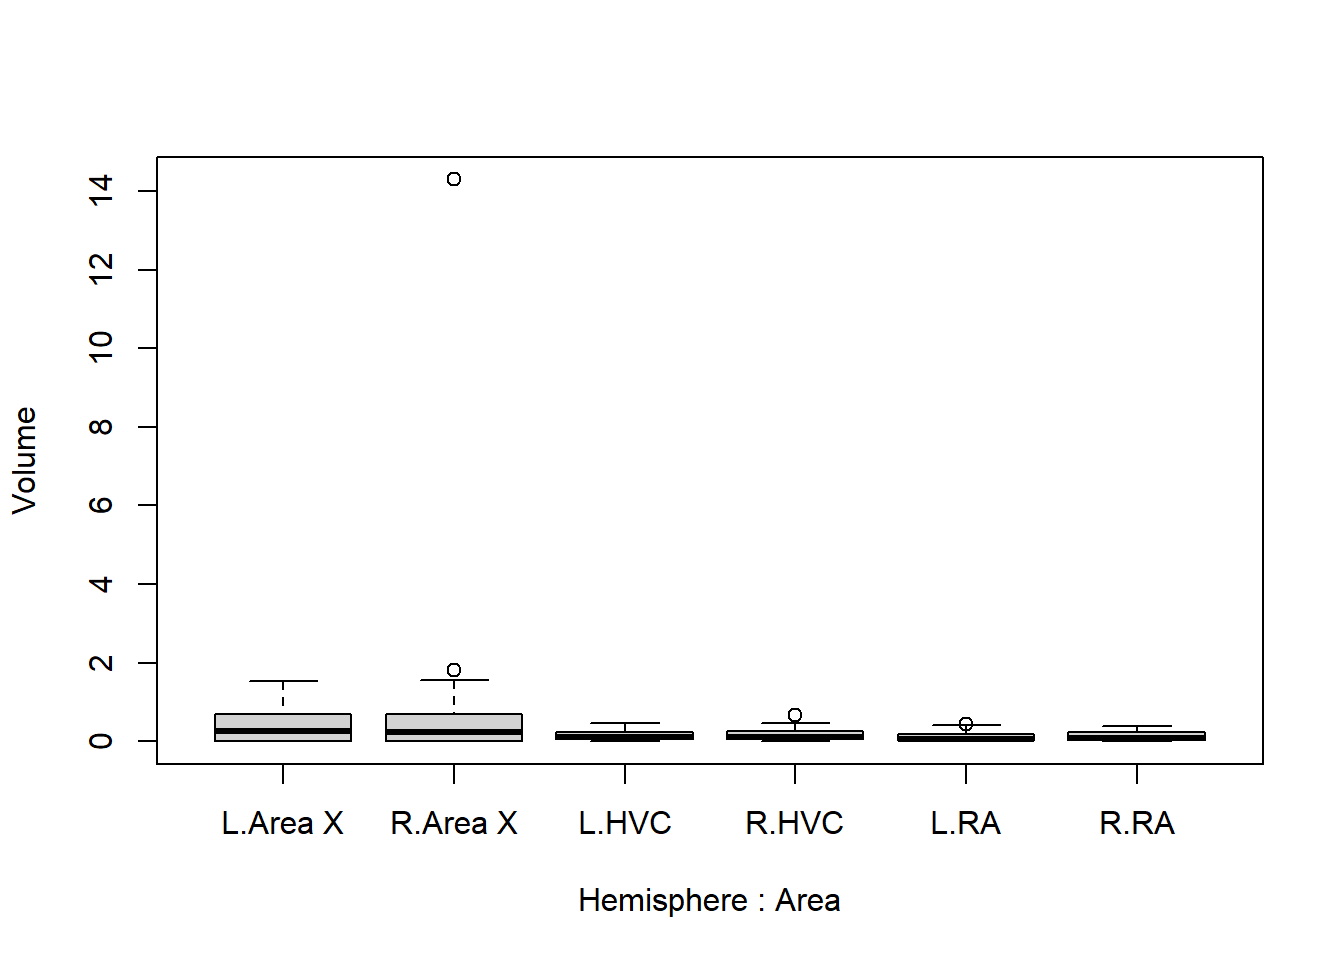
\includegraphics{Biostatistics_files/figure-latex/plot-1.pdf}

We can already make several useful observations:

\begin{itemize}
\tightlist
\item
  Area X seems to have a larger mean\footnote{If the mean is larger, the location of the boxplot is higher.} and variance\footnote{If the variance is larger, the size of the boxplot is larger.} than the rest;
\item
  The left and right hemispheres do not seem to differ much;
\item
  There is a suspiciously large value for area X of the right hemisphere. Is this an unrealistic value?
\end{itemize}

\hypertarget{inspect-suspicious-values}{%
\subsection{Inspect suspicious value(s)}\label{inspect-suspicious-values}}

Let's inspect the suspicious value further. Since it is the larger value, I can use \texttt{which.max} to find it:

\begin{Shaded}
\begin{Highlighting}[]
\NormalTok{suspicious <-}\StringTok{ }\KeywordTok{which.max}\NormalTok{(Birdsong}\OperatorTok{$}\NormalTok{Volume)}
\NormalTok{Birdsong}\OperatorTok{$}\NormalTok{Volume[suspicious] }\OperatorTok{/}\StringTok{ }\KeywordTok{mean}\NormalTok{(Birdsong}\OperatorTok{$}\NormalTok{Volume)}
\end{Highlighting}
\end{Shaded}

\begin{verbatim}
## [1] 53.86181
\end{verbatim}

This value is \(53.9 \times\) larger than the mean total volume. Keep in mind that volume is a three-dimensional measurement. It grows at a rate of \(x^3\) with the length, width and depth of the brain. Therefore, at least some extreme observations are expected\ldots{} So let's use a transformation that accounts for this:

\begin{Shaded}
\begin{Highlighting}[]
\KeywordTok{boxplot}\NormalTok{(Volume}\OperatorTok{^}\NormalTok{(}\DecValTok{1}\OperatorTok{/}\DecValTok{3}\NormalTok{) }\OperatorTok{~}\StringTok{ }\NormalTok{Hemisphere }\OperatorTok{*}\StringTok{ }\NormalTok{Area, }\DataTypeTok{data =}\NormalTok{ Birdsong)}
\end{Highlighting}
\end{Shaded}

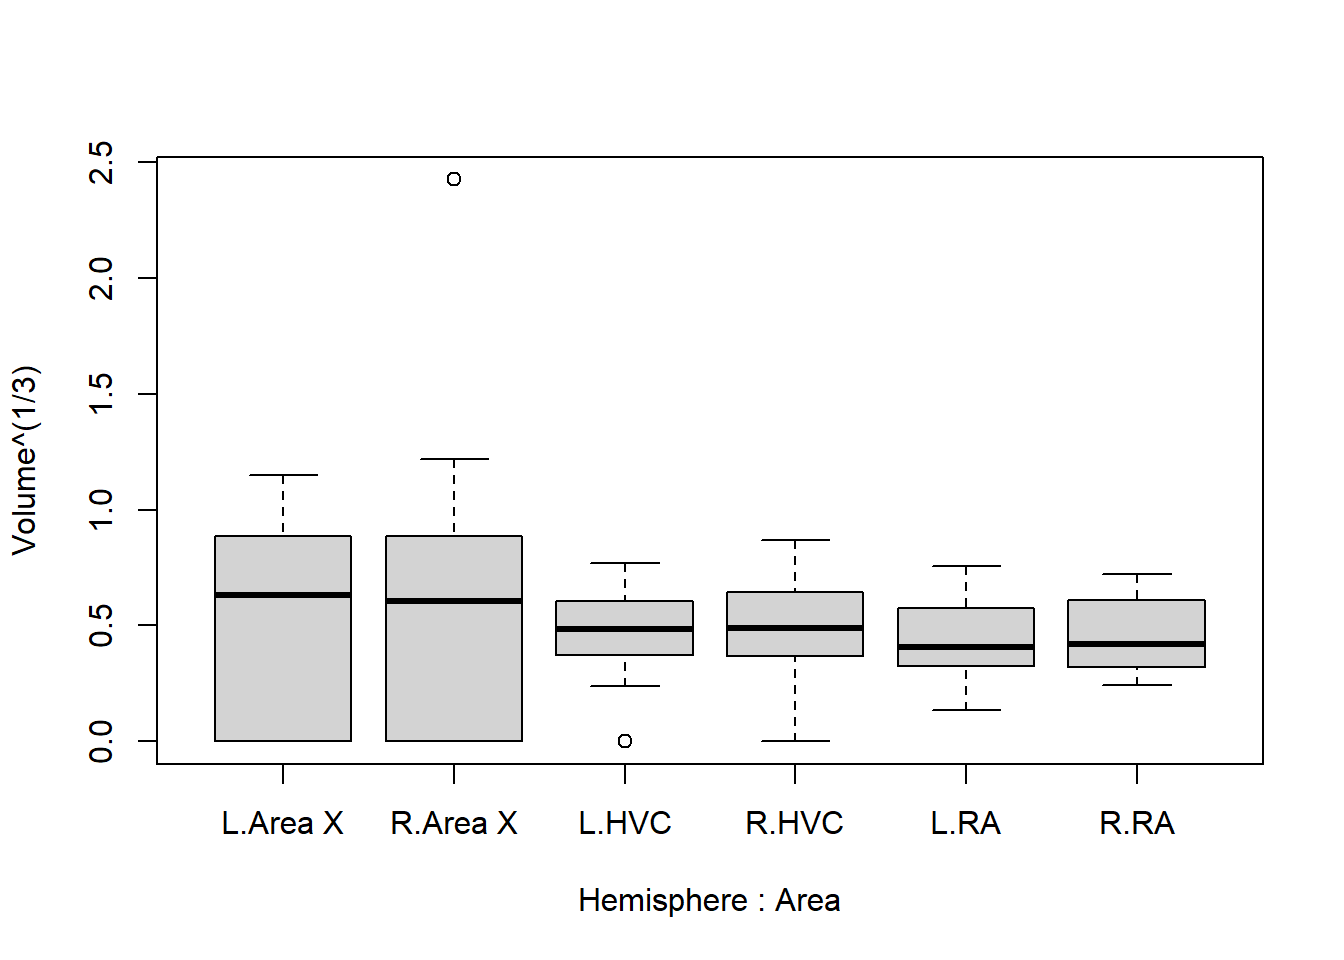
\includegraphics{Biostatistics_files/figure-latex/unnamed-chunk-15-1.pdf}

Even with a transformation of \(\text{volume}^\frac{1}{3}\), the suspiciously large value still sticks out quite a lot.

\hypertarget{remove-unrealistic-values}{%
\subsection{Remove unrealistic value(s)}\label{remove-unrealistic-values}}

It is hard to say what this value is supposed to be. It could have been a misplaced decimal separator, but should it then be \(1.4292\), or \(0.14292\)? Since we cannot say for sure what it should have been, let's omit this observation from further analysis:

\begin{Shaded}
\begin{Highlighting}[]
\NormalTok{Birdsong <-}\StringTok{ }\NormalTok{Birdsong[}\OperatorTok{-}\NormalTok{suspicious, ]}
\end{Highlighting}
\end{Shaded}

If this analysis were to be used in a publication, we would have to go further: How much does this observation affect the results? Can we use a form of multiple imputation to fill in the missing value we have now created? But for now we'll leave it at this.

Let's create the boxplots again to see what the data look like without the suspicious value:

\begin{Shaded}
\begin{Highlighting}[]
\KeywordTok{boxplot}\NormalTok{(Volume}\OperatorTok{^}\NormalTok{(}\DecValTok{1}\OperatorTok{/}\DecValTok{3}\NormalTok{) }\OperatorTok{~}\StringTok{ }\NormalTok{Hemisphere }\OperatorTok{*}\StringTok{ }\NormalTok{Area, }\DataTypeTok{data =}\NormalTok{ Birdsong)}
\end{Highlighting}
\end{Shaded}

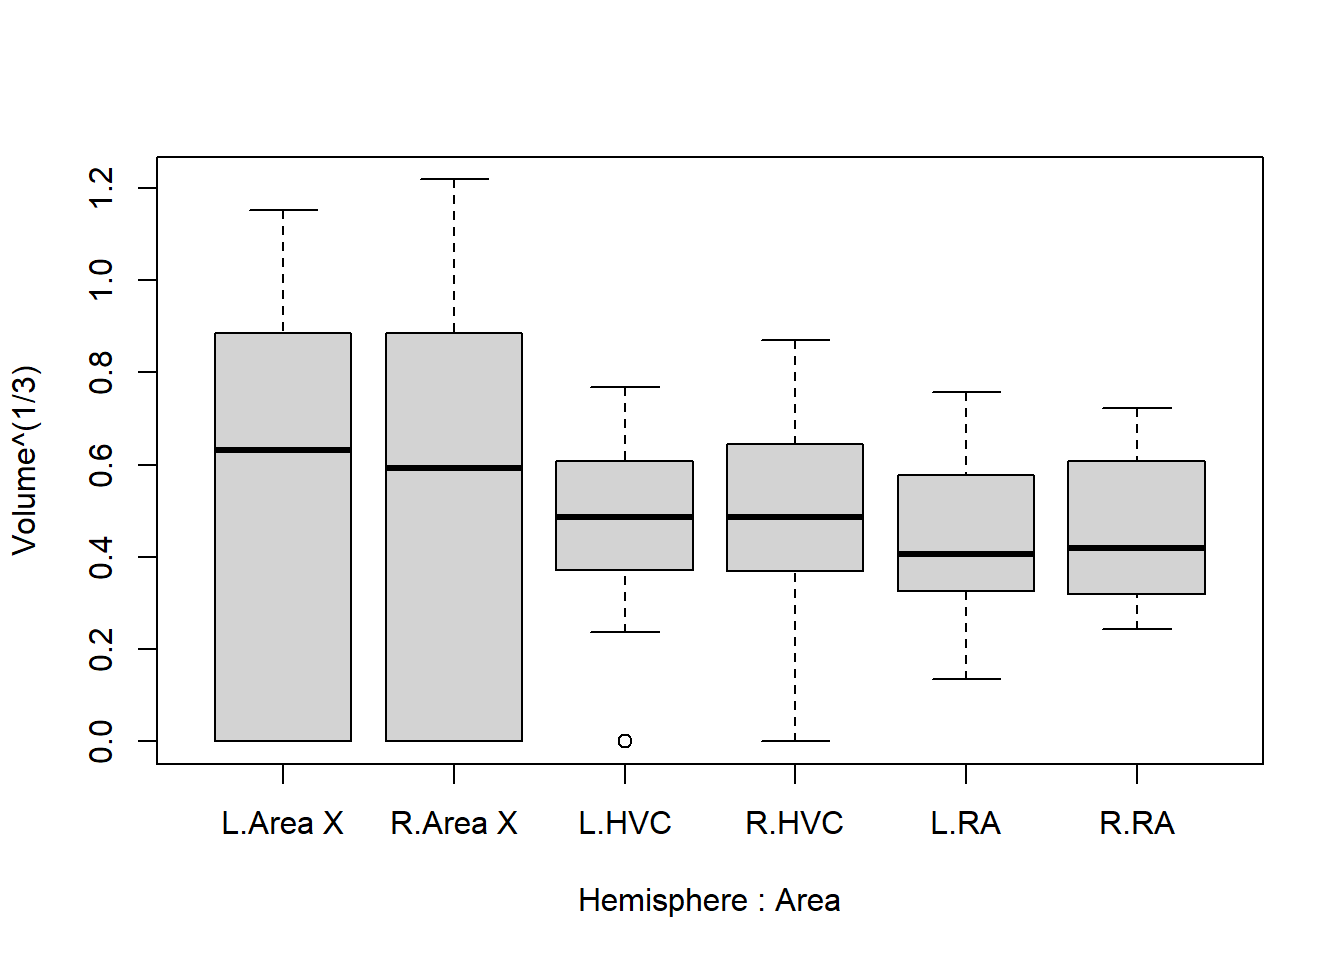
\includegraphics{Biostatistics_files/figure-latex/unnamed-chunk-17-1.pdf}

This looks far more reasonable. Now let's address the next elephant in the room: There appears to be far greater variance in the volume of area X, than in RA or HVC. But notice how measurements of zero almost exclusively occur in area X. We can confirm this as follows:

\begin{Shaded}
\begin{Highlighting}[]
\KeywordTok{by}\NormalTok{(Birdsong, Birdsong}\OperatorTok{$}\NormalTok{Area, }\ControlFlowTok{function}\NormalTok{(x)\{}\KeywordTok{sum}\NormalTok{(x }\OperatorTok{==}\StringTok{ }\DecValTok{0}\NormalTok{)\})}
\end{Highlighting}
\end{Shaded}

\begin{verbatim}
## Birdsong$Area: Area X
## [1] 45
## ------------------------------------------------------------ 
## Birdsong$Area: HVC
## [1] 8
## ------------------------------------------------------------ 
## Birdsong$Area: RA
## [1] 0
\end{verbatim}

How do we deal with this? There are several ways to do so, and the best way depends on the problem being studied, as well as the reason for measurements being \(0\). We could, for example, consider these zeroes to be `censored', meaning that they are not actually zero, but just too small to be picked up by the measurement. These kinds of considerations are what make statistical modeling difficult.

\hypertarget{remove-values-incorrectly-marked-0}{%
\subsection{Remove values incorrectly marked ``0''}\label{remove-values-incorrectly-marked-0}}

Fortunately, the cause of the zeroes was in most cases simply a low quality sample, unrelated to the actual volume. It is still suspicious that this happened considerably more often in area X than elsewhere, but for the purpose of this exercise let's consider these measurements to be missing completely at random. Whatever they were, they weren't \(0\), and this is skewing the results strongly otherwise.

Therefore, in the next step we set these values to `not available' (\texttt{NA}):

\begin{Shaded}
\begin{Highlighting}[]
\NormalTok{Birdsong}\OperatorTok{$}\NormalTok{Volume[Birdsong}\OperatorTok{$}\NormalTok{Volume }\OperatorTok{==}\StringTok{ }\DecValTok{0}\NormalTok{] <-}\StringTok{ }\OtherTok{NA}
\end{Highlighting}
\end{Shaded}

One final time we inspect the boxplots:

\begin{Shaded}
\begin{Highlighting}[]
\KeywordTok{boxplot}\NormalTok{(Volume}\OperatorTok{^}\NormalTok{(}\DecValTok{1}\OperatorTok{/}\DecValTok{3}\NormalTok{) }\OperatorTok{~}\StringTok{ }\NormalTok{Hemisphere }\OperatorTok{*}\StringTok{ }\NormalTok{Area, }\DataTypeTok{data =}\NormalTok{ Birdsong)}
\end{Highlighting}
\end{Shaded}

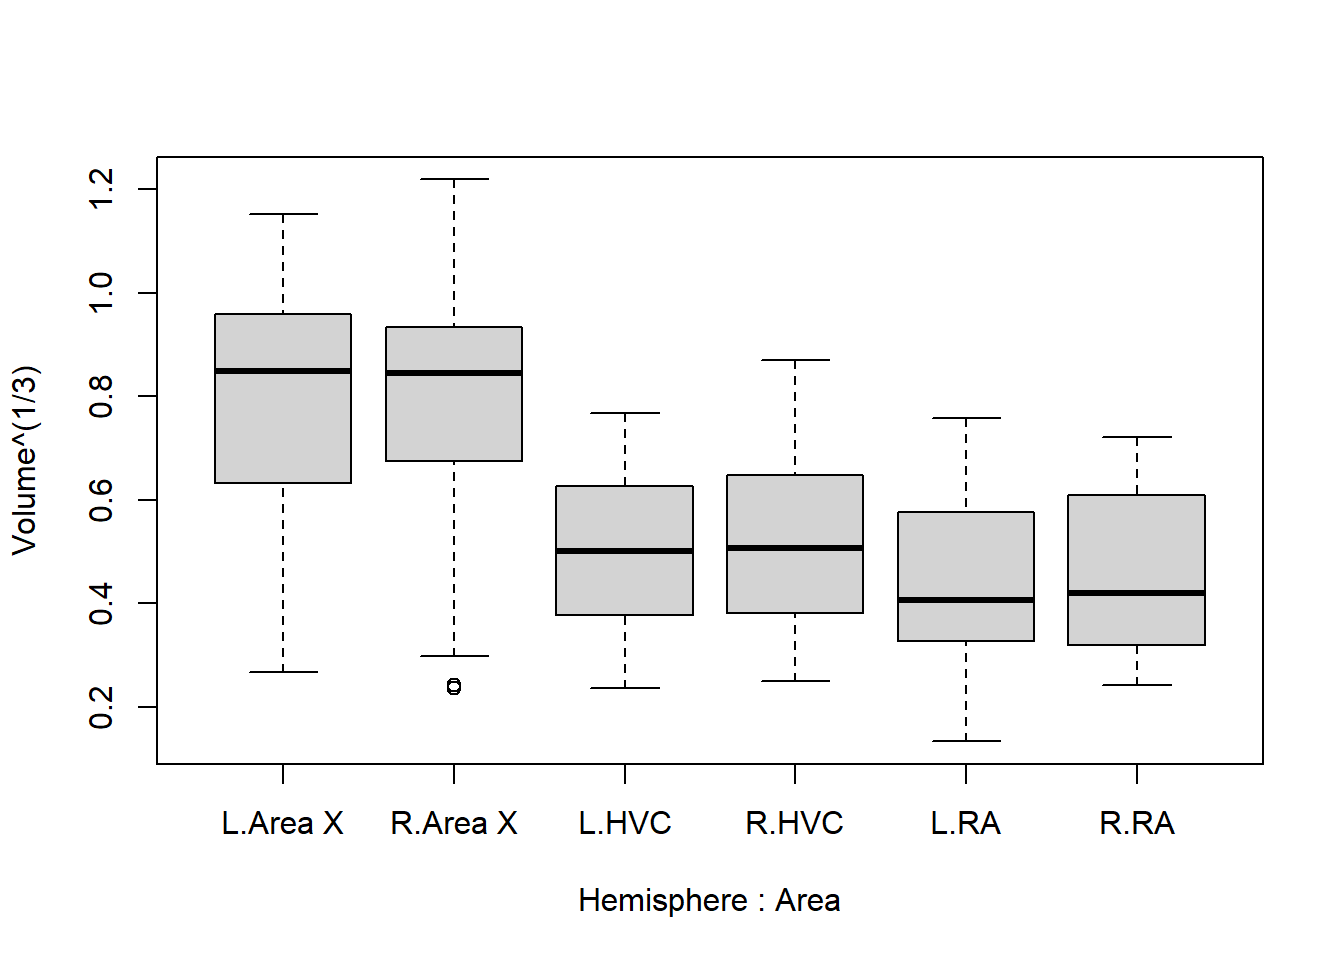
\includegraphics{Biostatistics_files/figure-latex/unnamed-chunk-20-1.pdf}

And now we have a fairly good idea of what we should expect in the results: HVC is lower than area X, and RA is even lower. The difference between hemispheres is extremely small and unlikely to be picked up by the model.

\hypertarget{other-changes}{%
\subsection{Other changes}\label{other-changes}}

Are there any other strange values, incorrect labels, or other problems in your version of the data set? Adjust the data in R as you see fit before moving on to the analysis.

\hypertarget{run-the-analysis}{%
\subsection{Run the analysis}\label{run-the-analysis}}

Once you're over here, you can copy the models I've \protect\hyperlink{brainmodel}{shown above}:

\begin{Shaded}
\begin{Highlighting}[]
\NormalTok{model1 <-}\StringTok{ }\KeywordTok{lmer}\NormalTok{(Volume}\OperatorTok{^}\NormalTok{(}\DecValTok{1}\OperatorTok{/}\DecValTok{3}\NormalTok{) }\OperatorTok{~}\StringTok{ }\NormalTok{Area }\OperatorTok{+}\StringTok{ }\NormalTok{Hemisphere }\OperatorTok{+}\StringTok{ }\NormalTok{(}\DecValTok{1} \OperatorTok{|}\StringTok{ }\NormalTok{BirdID) }\OperatorTok{+}\StringTok{ }\NormalTok{(}\DecValTok{1} \OperatorTok{|}\StringTok{ }\NormalTok{StudentID), }
               \DataTypeTok{data =}\NormalTok{ Birdsong)}
\NormalTok{model2 <-}\StringTok{ }\KeywordTok{lmer}\NormalTok{(Volume}\OperatorTok{^}\NormalTok{(}\DecValTok{1}\OperatorTok{/}\DecValTok{3}\NormalTok{) }\OperatorTok{~}\StringTok{ }\NormalTok{Area }\OperatorTok{+}\StringTok{ }\NormalTok{Hemisphere }\OperatorTok{+}\StringTok{ }\NormalTok{(}\DecValTok{1} \OperatorTok{|}\StringTok{ }\NormalTok{BirdID), }
               \DataTypeTok{data =}\NormalTok{ Birdsong)}
\end{Highlighting}
\end{Shaded}

Do both models run without errors? Can you \protect\hyperlink{comparebrain}{compare the models like shown before}? What do you conclude from \protect\hyperlink{brainoutput}{the output}?

\end{document}
